\documentclass[a4paper, 12pt]{article}
% math symbols
\usepackage{amssymb}
\usepackage{amsmath}
\usepackage{mathrsfs}
\usepackage{physsummer}


\usepackage{enumitem}
\usepackage[margin = 2cm]{geometry}

\tolerance = 1000
\emergencystretch = 0.74cm



\pagestyle{empty}
\parindent = 0mm

\usetikzlibrary{hobby}

\begin{document}

\begin{center}
  \Large{\textbf{Городской центр физического образования, 10 класс.}\\
  \textit{Серия 5, 16 октября 2014.}}
\end{center}

\begin{center}
  \Large \textbf{ Давление в газах.}
\end{center}

\Large

\task{ Цилиндрический сосуд с идеальным газом разделен подвижным
  поршнем на две части. Газ в левом отделении нагревают до температуры
  $T_1$, а в правом до температуры $T_2$. При этом соотношение объёмов
  оказывается равным $V_1/V_2=2$. После того как температуры
  выравнялись, соотношение объёмов изменилось:
  $V_1/V_2=1/2$. Определите отношение температур $T_1/T_2$.  }

\taskpic{ Перевёрнутый цилиндрический стакан высотой $H$ аккуратно
  погружен в жидкость плотностью $\rho$ так, что в жидкости находится
  2/3 стакана. Чему равно атмосферное давление, если жидкость
  поднялась в стакан на высоту $h$? } {
  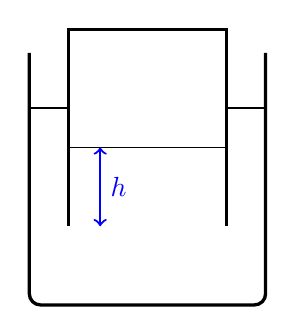
\begin{tikzpicture}
    \draw[very thick,rounded corners] (0,3.2) -- (0,0) -- (3,0) --
    (3,3.2); 
    \draw[thick] (0,2.5) -- (3,2.5);
    \draw[black, fill=white] (0.5,2) rectangle (2.5,3.5);
    \draw[very thick] (0.5,1) -- (0.5,3.5) -- (2.5,3.5) -- (2.5,1);
    \draw[blue, thick, <->] (0.9,1) -- (0.9,2) node[midway,right] {$h$}; 
  \end{tikzpicture}
}

\task{ Герметично закрытый сосуд заполнили водой плотностью $\rho$
  так, что на дне сосуда остался пузырёк воздуха. Как изменится
  давление воды на дно сосуда, если пузырек всплывет? Высота сосуда
  $h$. Считать процесс изотермическим. }

\end{document}


%%% Local Variables: 
%%% mode: latex
%%% TeX-engine:xetex
%%% TeX-PDF-mode: t
%%% End:
